\chapter{晶体 II：离子固体、共价固体与分子固体}\label{ch:b1:crystals-ionic-covalent}

研碎的食盐会碎裂成细小的立方体；金刚石是最硬的
天然材料，而由同样的碳原子构成的石墨却很软，
软到可以用来写字；冰会漂浮在水面上。它们都是晶体，但其
粒子以不同的方式结合在一起：离子依靠静电
吸引，原子依靠共价键，分子依靠分子间
作用力结合（见\cref{ch:b1:intermolecular-forces-solvents}）。本章
将上一章的晶胞几何应用于这三类
固体，并从离子的大小解释氯化钠
与氯化铯为何采取不同的结构。

\begin{recall}
晶胞的微观态数、配位数与堆积率，以及
面心立方晶格的八面体间隙与四面体间隙，均已
在\cref{ch:b1:crystals-metals}中定义；晶体的密度为
$\rho = ZM/(N_A V)$（见\cref{prop:b1:crystals-metals:density}）。离子半径
已在\cref{def:b1:periodicity:radius}中引入。
\end{recall}

\section{离子晶体与半径比}

\begin{definition}[离子晶体]\label{def:b1:crystals-ionic-covalent:ionic-crystal}
称\emph{离子晶体}\index{离子晶体}为由阳离子与
阴离子通过静电吸引结合而成的晶体。每个离子
被电荷相反的离子包围；晶体呈电中性，因此晶胞中
阳离子与阴离子的数目之比等于化学式中的比例。
\end{definition}

\begin{proposition}[离子晶体的性质]\label{prop:b1:crystals-ionic-covalent:ionic-properties}
离子晶体硬而脆（一层发生位移时，
同号离子面对面，晶体便会解理），具有较高的熔
点，固态时不导电，熔融或溶解后导电，
并能溶于介电常数高的极性溶剂。
\end{proposition}
\admitted

\begin{definition}[半径比]\label{def:b1:crystals-ionic-covalent:radius-ratio}
在阳离子半径为 $r_+$、阴离子半径为
$r_-$ 的离子晶体中，称\emph{半径比}\index{半径比}为 $x = r_+/r_-$
（通常 $x < 1$，阳离子比阴离子小）。
\end{definition}

\begin{proposition}[半径比规则]\label{prop:b1:crystals-ionic-covalent:rule}
在硬球模型中，若每个阳离子与 $n$
个阴离子接触，则该结构稳定，当且仅当阴离子之间互不接触，
这要求 $x$ 高于由几何决定的下限：$x \ge \sqrt3 - 1
\approx 0.732$ 对应 8 个近邻（立方体），$x \ge \sqrt2 - 1 \approx 0.414$
对应 6 个（八面体），$x \ge \sqrt{3/2} - 1 \approx 0.225$ 对应 4
个（四面体）。所采取的结构是 $x$ 所允许的
配位数最高的那一种。
\end{proposition}

\begin{proof}
阳离子位于与其接触的 $n$ 个阴离子之间的空隙中。在
极限情形下，阴离子之间也相互接触。立方体情形：阴离子位于
边长为 $2r_-$ 的立方体顶点上，阳离子位于其中心，因此 $r_+ +
r_- = \sqrt3\,r_-$。八面体情形：四个阴离子位于边长为 $2r_-$ 的正方形
的顶点上，阳离子位于其中心，$r_+ + r_- = \sqrt2\,r_-$。四面体情形：
阴离子位于边长为 $\sqrt2\,r_-$ 的立方体交替顶点上，阳离子位于
中心，$r_+ + r_- = \frac{\sqrt3}{2}\sqrt2\,r_- = \sqrt{3/2}\,r_-$。
除以 $r_-$ 即得上述下限。低于下限时，阳离子在
过大的空隙中晃动：阴离子相互排斥，而吸引作用并未增强，
因此配位数较低、空隙较小的结构更为稳定。
\end{proof}

\begin{omfigure}
\begin{tikzpicture}[font=\small, >={Stealth}]
  \draw[->, thick] (0,0) -- (12.4,0) node[right] {$x = r_+/r_-$};
  \foreach \x/\l in {0/0, 2.7/0.225, 4.97/0.414, 8.78/0.732, 12/1} {
    \draw (\x,0.12) -- (\x,-0.12) node[below] {\l};
  }
  \fill[omDef!15] (2.7,0.2) rectangle (4.97,1.0);
  \fill[omProp!15] (4.97,0.2) rectangle (8.78,1.0);
  \fill[omThm!15] (8.78,0.2) rectangle (12,1.0);
  \node[align=center] at (3.83,0.6) {4：闪锌矿型};
  \node[align=center] at (6.87,0.6) {6：氯化钠型};
  \node[align=center] at (10.4,0.6) {8：氯化铯型};
  \foreach \x/\l in {3.91/\ce{ZnS}, 6.76/\ce{NaCl}, 10.08/\ce{RbCl}, 11.54/\ce{CsCl}} {
    \draw[omExo, thick] (\x,-0.55) -- (\x,-0.95);
    \node[below, omExo] at (\x,-0.95) {\l};
  }
\end{tikzpicture}

{\small 半径比规则：阳离子的配位数
由 $x$ 所允许，并给出四种盐的实测比值（香农半径）。
氯化铷的比值为 0.84，按理应属 \ce{CsCl} 型，但
实际采取 \ce{NaCl} 型：该规则只是指导，而非定律
（见\cref{exo:b1:crystals-ionic-covalent:12}）。}
% ledger: rion:Zn2+IV, rion:S2-VI, rion:Na+VI, rion:Cl-VI, rion:Rb+VI,
% rion:Cs+VIII
\end{omfigure}

\section{四种结构类型}

\begin{definition}[结构类型]\label{def:b1:crystals-ionic-covalent:structure-type}
离子晶体可按少数几种结构类型加以分类，这些类型以一种
代表性化合物命名：
\begin{itemize}
  \item \emph{氯化铯型}\index{氯化铯型}：阴离子
        位于立方体的顶点，阳离子位于其中心（8:8）；
  \item \emph{氯化钠型}\index{氯化钠型}
        ：阴离子位于面心立方晶格上，阳离子占据其全部
        八面体间隙（6:6）；
  \item \emph{闪锌矿型}\index{闪锌矿型}：阴离子位于面心立方
        晶格上，阳离子占据其四面体间隙的一半，每隔一个交替
        占据（4:4）；
  \item \emph{萤石型}\index{萤石型}：阳离子位于面心立方
        晶格上，阴离子占据其全部四面体间隙（8:4），化学式为
        \ce{MX2}；在\emph{反萤石型}\index{反萤石型}中
        两者角色互换（\ce{Li2O}，4:8）。
\end{itemize}
数对给出阳离子与
阴离子的配位数。
\end{definition}

\begin{omfigure}
\tdplotsetmaincoords{60}{100}
\begin{tikzpicture}[tdplot_main_coords, font=\small]
  \pic {omcubeo={3}};
    \node[aX={green!55!black}{6.5mm}] at (0,0,0) {};
  \node[aX={violet!70}{3.8mm}] at (0,1.5,0) {};
  \node[aX={green!55!black}{6.5mm}] at (0,3,0) {};
  \node[aX={violet!70}{3.8mm}] at (0,0,1.5) {};
  \node[aX={green!55!black}{6.5mm}] at (0,1.5,1.5) {};
  \node[aX={violet!70}{3.8mm}] at (0,3,1.5) {};
  \node[aX={violet!70}{3.8mm}] at (1.5,0,0) {};
  \node[aX={green!55!black}{6.5mm}] at (0,0,3) {};
  \node[aX={green!55!black}{6.5mm}] at (1.5,1.5,0) {};
  \node[aX={violet!70}{3.8mm}] at (0,1.5,3) {};
  \node[aX={violet!70}{3.8mm}] at (1.5,3,0) {};
  \node[aX={green!55!black}{6.5mm}] at (0,3,3) {};
  \node[aX={green!55!black}{6.5mm}] at (1.5,0,1.5) {};
  \node[aX={violet!70}{3.8mm}] at (1.5,1.5,1.5) {};
  \node[aX={green!55!black}{6.5mm}] at (1.5,3,1.5) {};
  \node[aX={green!55!black}{6.5mm}] at (3,0,0) {};
  \node[aX={violet!70}{3.8mm}] at (1.5,0,3) {};
  \node[aX={violet!70}{3.8mm}] at (3,1.5,0) {};
  \node[aX={green!55!black}{6.5mm}] at (1.5,1.5,3) {};
  \node[aX={green!55!black}{6.5mm}] at (3,3,0) {};
  \node[aX={violet!70}{3.8mm}] at (1.5,3,3) {};
  \node[aX={violet!70}{3.8mm}] at (3,0,1.5) {};
  \node[aX={green!55!black}{6.5mm}] at (3,1.5,1.5) {};
  \node[aX={violet!70}{3.8mm}] at (3,3,1.5) {};
  \node[aX={green!55!black}{6.5mm}] at (3,0,3) {};
  \node[aX={violet!70}{3.8mm}] at (3,1.5,3) {};
  \node[aX={green!55!black}{6.5mm}] at (3,3,3) {};
  \node at (1.5,1.5,-1.75) {\ce{NaCl}（氯化钠型）};
\end{tikzpicture}
\hspace{1cm}
\begin{tikzpicture}[tdplot_main_coords, font=\small]
  \pic {omcubeo={3}};
    \node[aX={green!55!black}{6.5mm}] at (0,0,0) {};
  \node[aX={green!55!black}{6.5mm}] at (0,3,0) {};
  \node[aX={green!55!black}{6.5mm}] at (0,0,3) {};
  \node[aX={green!55!black}{6.5mm}] at (0,3,3) {};
  \node[aX={blue!60}{7mm}] at (1.5,1.5,1.5) {};
  \node[aX={green!55!black}{6.5mm}] at (3,0,0) {};
  \node[aX={green!55!black}{6.5mm}] at (3,3,0) {};
  \node[aX={green!55!black}{6.5mm}] at (3,0,3) {};
  \node[aX={green!55!black}{6.5mm}] at (3,3,3) {};
  \node at (1.5,1.5,-1.75) {\ce{CsCl}（氯化铯型）};
\end{tikzpicture}

{\small 左：氯化钠型晶胞，\ce{Cl-}（绿色）位于面心立方晶格上，
\ce{Na+}（紫色）占据每个八面体间隙。右：氯化铯型晶胞，
\ce{Cl-}位于顶点，\ce{Cs+}（蓝色）位于晶胞中心。离子画得
比相切时小。}
\end{omfigure}

\begin{proposition}[氯化钠型与氯化铯型]\label{prop:b1:crystals-ionic-covalent:nacl-cscl}
在氯化钠型中，每个晶胞含 $Z = 4$ 个化学式单位，离子
沿棱相切，$a = 2(r_+ + r_-)$，且结构要求 $\sqrt2 - 1
\le x$。在氯化铯型中，$Z = 1$，离子沿
体对角线相切，$a\sqrt3 = 2(r_+ + r_-)$，且结构要求
$x \ge \sqrt3 - 1$。
\end{proposition}

\begin{proof}
氯化钠型：面心立方晶格上的阴离子数为 $4$，八面体间隙中的阳离子数为
$1 + 12 \times \frac14 = 4$。沿棱方向，阴离子、
阳离子与阴离子依次相接。阴离子不重叠，须
面对角线（含三个阴离子，其中至多两个相接）满足
$a\sqrt2 \ge 4r_-$，即 $2(r_+ + r_-)\sqrt2 \ge
4r_-$，亦即 $x \ge \sqrt2 - 1$。氯化铯型：$8 \times \frac18 = 1$
个阴离子和 1 个阳离子；沿体对角线依次为阴离子、阳离子、阴离子相接；
若沿棱方向阴离子不重叠，须 $a \ge 2r_-$，即
$2(r_+ + r_-)/\sqrt3 \ge 2r_-$，亦即 $x \ge \sqrt3 - 1$。
\end{proof}

\begin{example}[氯化钠与氯化铯]\label{ex:b1:crystals-ionic-covalent:nacl}
氯化钠的 $a = \qty{564.1}{pm}$：$r_+ + r_- = a/2 =
\qty{282.0}{pm}$，与香农半径给出的 $102 + 181 = \qty{283}{pm}$ 相比；
$x = 102/181 = 0.56$，位于八面体范围内。其密度为
$\rho = 4 \times 58.44/(6.022 \times 10^{23} \times (5.641 \times
10^{-8})^3) = \qty{2.16}{g/cm^3}$，实测为 \qty{2.17}{g/cm^3}。
氯化铯的 $a = \qty{412.3}{pm}$：$r_+ + r_- = a\sqrt3/2 =
\qty{357.1}{pm}$，且 $x = 174/181 = 0.96$，位于立方范围内。
% ledger: lat:NaCl, rion:Na+VI, rion:Cl-VI, rho:NaCl, lat:CsCl,
% rion:Cs+VIII
\end{example}

\begin{omfigure}
\begin{minipage}[b]{0.31\linewidth}\centering
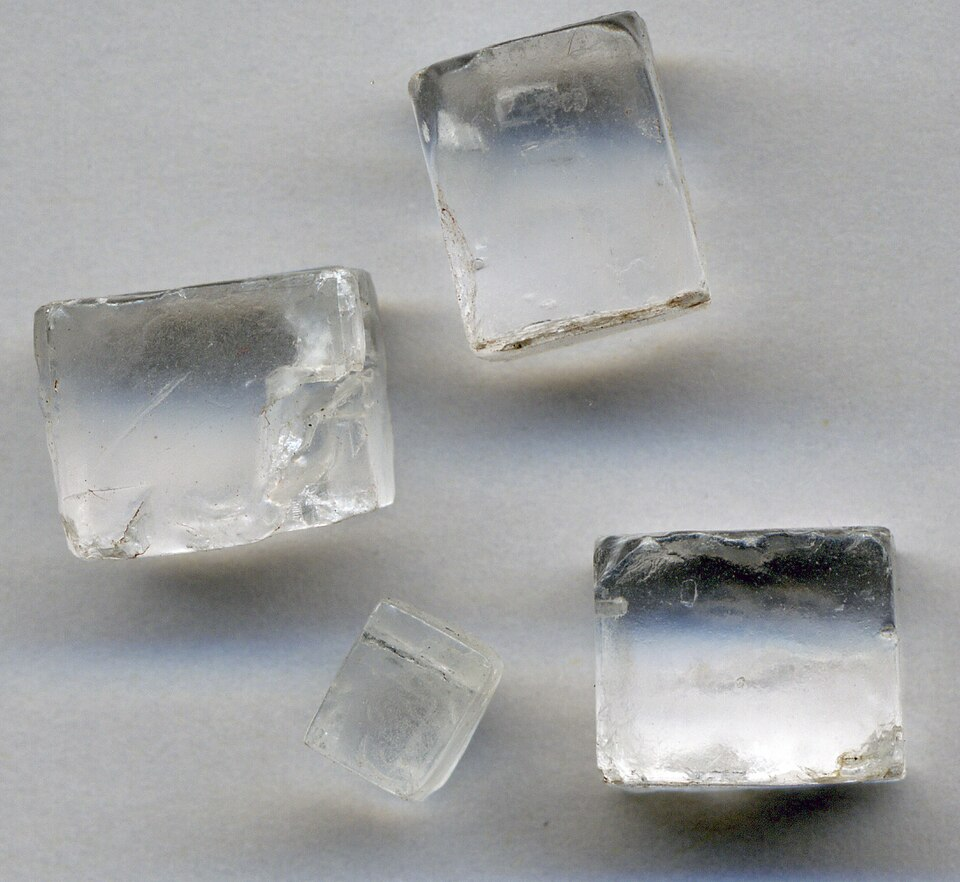
\includegraphics[width=\linewidth]{images/book2/halite.jpg}

{\small 石盐（氯化钠型）晶体。照片：James St. John，CC BY 2.0。}
\end{minipage}\hfill
\begin{minipage}[b]{0.31\linewidth}\centering
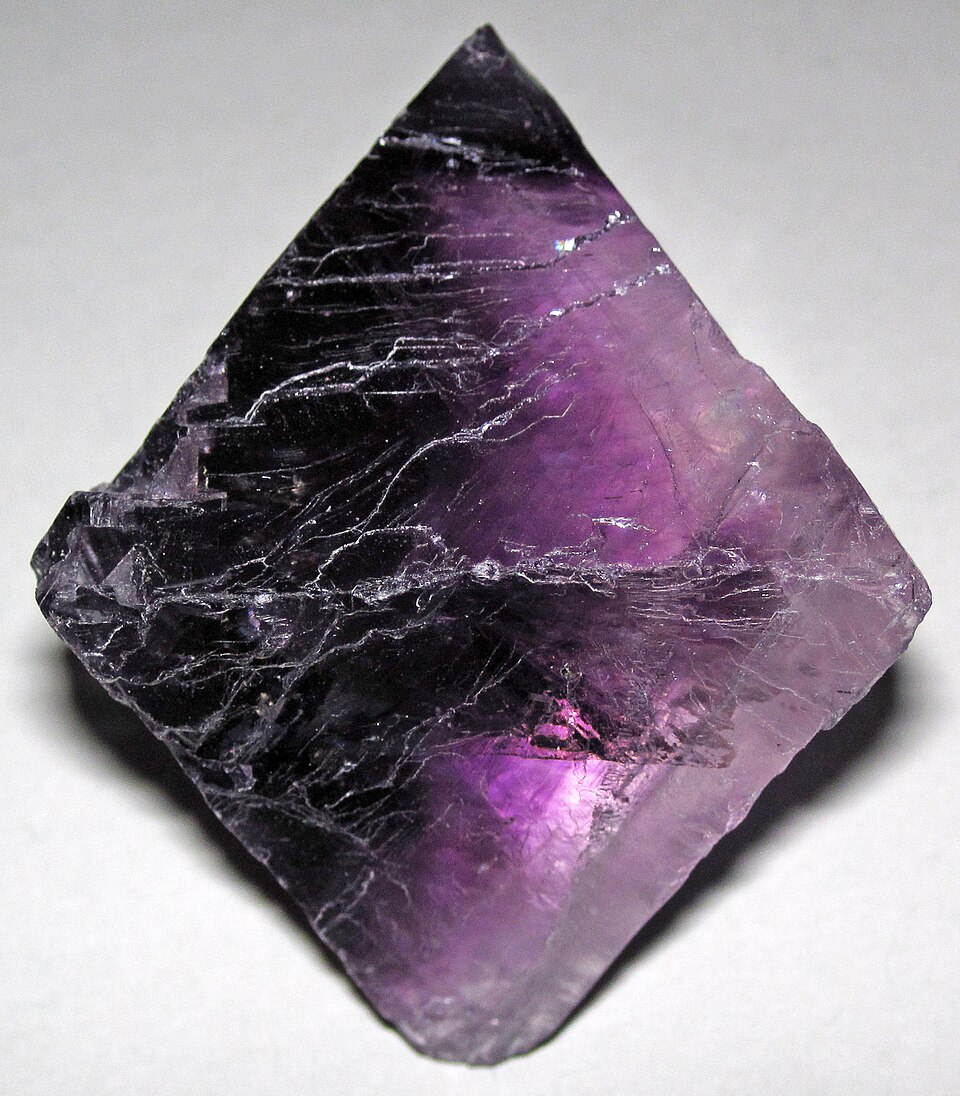
\includegraphics[width=0.85\linewidth]{images/book2/fluorite.jpg}

{\small 萤石，\ce{CaF2}。照片：James St. John，CC BY 2.0。}
\end{minipage}\hfill
\begin{minipage}[b]{0.31\linewidth}\centering
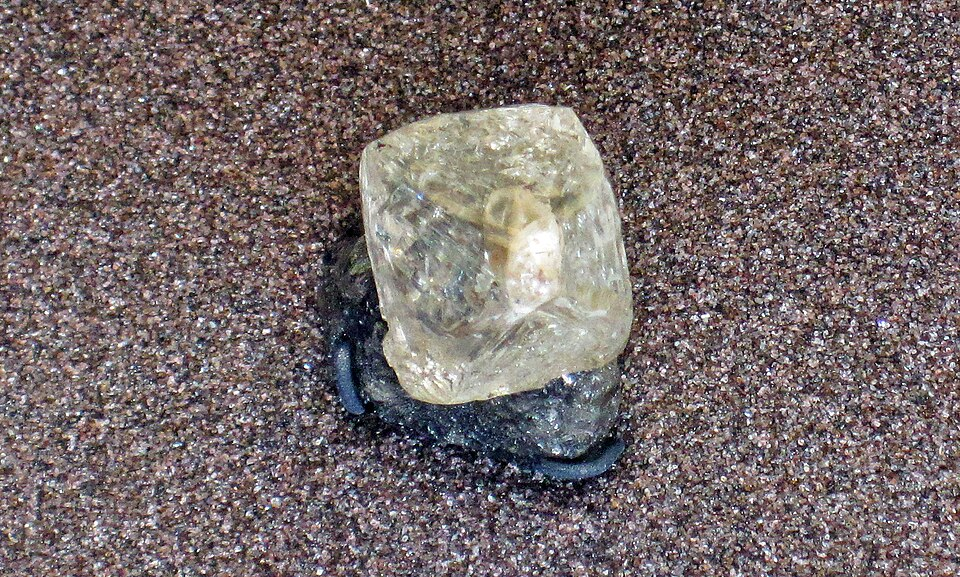
\includegraphics[width=\linewidth]{images/book2/diamond.jpg}

{\small 一颗粗糙的金刚石八面体。照片：James St. John，CC BY 2.0。}
\end{minipage}
\end{omfigure}

\begin{proposition}[闪锌矿型与萤石型]\label{prop:b1:crystals-ionic-covalent:zns-caf2}
在闪锌矿型中，$Z = 4$，每个离子被四个异种离子
包围，这些离子位于四面体的顶点，离子沿体对角线的
四分之一相切：$a\sqrt3/4 = r_+ + r_-$。在萤石型中，
$Z = 4$ 个 \ce{CaF2} 单位，每个阳离子有 8 个阴离子近邻（组成立方体），
每个阴离子有 4 个阳离子近邻（组成四面体），且同样有 $a\sqrt3/4 =
r_+ + r_-$。
\end{proposition}

\begin{proof}
闪锌矿型：4 个阴离子位于面心立方晶格上，4 个阳离子占据
8 个四面体间隙中的一半。位于 $(\frac a4,\frac a4,\frac a4)$ 的
四面体间隙与其四个阴离子的距离为 $\frac{a\sqrt3}{4}$。萤石型：4 个阳离子和
8 个阴离子占据全部四面体间隙，比例为 $1:2$。晶胞内的 8 个阴离子
构成棱长为 $a/2$ 的立方体，每隔一个小立方体的中心放一个阳离子；
每个阴离子的 4 个阳离子近邻位于
$\frac{a\sqrt3}{4}$ 处。
\end{proof}

\begin{omfigure}
\tdplotsetmaincoords{60}{100}
\begin{tikzpicture}[tdplot_main_coords, font=\small]
  \pic {omcubeo={3}};
  \begin{scope}[on background layer]
    \draw[black!45, line width=1.2pt] (0.75,0.75,2.25) -- (0,0,3) (0.75,0.75,2.25) -- (0,1.5,1.5) (0.75,0.75,2.25) -- (1.5,0,1.5) (0.75,0.75,2.25) -- (1.5,1.5,3) (0.75,2.25,0.75) -- (0,1.5,1.5) (0.75,2.25,0.75) -- (0,3,0) (0.75,2.25,0.75) -- (1.5,1.5,0) (0.75,2.25,0.75) -- (1.5,3,1.5) (2.25,0.75,0.75) -- (1.5,0,1.5) (2.25,0.75,0.75) -- (1.5,1.5,0) (2.25,0.75,0.75) -- (3,0,0) (2.25,0.75,0.75) -- (3,1.5,1.5) (2.25,2.25,2.25) -- (1.5,1.5,3) (2.25,2.25,2.25) -- (1.5,3,1.5) (2.25,2.25,2.25) -- (3,1.5,1.5) (2.25,2.25,2.25) -- (3,3,3);
  \end{scope}
    \node[aX={yellow!75!orange}{6mm}] at (0,0,0) {};
  \node[aX={yellow!75!orange}{6mm}] at (0,3,0) {};
  \node[aX={yellow!75!orange}{6mm}] at (0,1.5,1.5) {};
  \node[aX={gray!60}{3.6mm}] at (0.75,2.25,0.75) {};
  \node[aX={yellow!75!orange}{6mm}] at (0,0,3) {};
  \node[aX={yellow!75!orange}{6mm}] at (1.5,1.5,0) {};
  \node[aX={gray!60}{3.6mm}] at (0.75,0.75,2.25) {};
  \node[aX={yellow!75!orange}{6mm}] at (0,3,3) {};
  \node[aX={yellow!75!orange}{6mm}] at (1.5,0,1.5) {};
  \node[aX={gray!60}{3.6mm}] at (2.25,0.75,0.75) {};
  \node[aX={yellow!75!orange}{6mm}] at (1.5,3,1.5) {};
  \node[aX={yellow!75!orange}{6mm}] at (3,0,0) {};
  \node[aX={yellow!75!orange}{6mm}] at (1.5,1.5,3) {};
  \node[aX={yellow!75!orange}{6mm}] at (3,3,0) {};
  \node[aX={gray!60}{3.6mm}] at (2.25,2.25,2.25) {};
  \node[aX={yellow!75!orange}{6mm}] at (3,1.5,1.5) {};
  \node[aX={yellow!75!orange}{6mm}] at (3,0,3) {};
  \node[aX={yellow!75!orange}{6mm}] at (3,3,3) {};
  \node at (1.5,1.5,-1.75) {\ce{ZnS} （闪锌矿型）};
\end{tikzpicture}
\hspace{1cm}
\begin{tikzpicture}[tdplot_main_coords, font=\small]
  \pic {omcubeo={3}};
    \node[aX={green!35!gray}{4.4mm}] at (0,0,0) {};
  \node[aX={green!35!gray}{4.4mm}] at (0,3,0) {};
  \node[aX={green!35!gray}{4.4mm}] at (0,1.5,1.5) {};
  \node[aX={green!45!yellow}{5.0mm}] at (0.75,0.75,0.75) {};
  \node[aX={green!45!yellow}{5.0mm}] at (0.75,2.25,0.75) {};
  \node[aX={green!35!gray}{4.4mm}] at (0,0,3) {};
  \node[aX={green!35!gray}{4.4mm}] at (1.5,1.5,0) {};
  \node[aX={green!45!yellow}{5.0mm}] at (0.75,0.75,2.25) {};
  \node[aX={green!35!gray}{4.4mm}] at (0,3,3) {};
  \node[aX={green!35!gray}{4.4mm}] at (1.5,0,1.5) {};
  \node[aX={green!45!yellow}{5.0mm}] at (0.75,2.25,2.25) {};
  \node[aX={green!45!yellow}{5.0mm}] at (2.25,0.75,0.75) {};
  \node[aX={green!35!gray}{4.4mm}] at (1.5,3,1.5) {};
  \node[aX={green!35!gray}{4.4mm}] at (3,0,0) {};
  \node[aX={green!45!yellow}{5.0mm}] at (2.25,2.25,0.75) {};
  \node[aX={green!35!gray}{4.4mm}] at (1.5,1.5,3) {};
  \node[aX={green!35!gray}{4.4mm}] at (3,3,0) {};
  \node[aX={green!45!yellow}{5.0mm}] at (2.25,0.75,2.25) {};
  \node[aX={green!45!yellow}{5.0mm}] at (2.25,2.25,2.25) {};
  \node[aX={green!35!gray}{4.4mm}] at (3,1.5,1.5) {};
  \node[aX={green!35!gray}{4.4mm}] at (3,0,3) {};
  \node[aX={green!35!gray}{4.4mm}] at (3,3,3) {};
  \node at (1.5,1.5,-1.75) {\ce{CaF2} （萤石型）};
\end{tikzpicture}

{\small 左：闪锌矿型，\ce{S^{2-}}（黄色）位于面心立方晶格上，
\ce{Zn^{2+}}（灰色）位于隔一个的四面体间隙中，每个都与其四个近邻相连。
右：萤石型，\ce{Ca^{2+}}（灰绿色）位于面心立方晶格上，
\ce{F-}（浅绿色）位于全部八个四面体间隙中。}
\end{omfigure}

\begin{example}[闪锌矿型与萤石型]\label{ex:b1:crystals-ionic-covalent:zns}
闪锌矿型的 $a = \qty{540.9}{pm}$，$r_+ + r_- = a\sqrt3/4 =
\qty{234.2}{pm}$（香农半径：$60 + 184 = \qty{244}{pm}$，硫化物半径
仅在六配位时列出），且 $x = 60/184 = 0.33$，位于
四面体范围内。萤石型的 $a = \qty{546.3}{pm}$，$r_+ + r_- =
\qty{236.6}{pm}$（香农半径：$112 + 131 = \qty{243}{pm}$），且 $x = 0.85$：
阳离子位于由 8 个阴离子构成的立方体中，与该规则相符。
% ledger: lat:ZnS, rion:Zn2+IV, rion:S2-VI, lat:CaF2, rion:Ca2+VIII,
% rion:F-IV
\end{example}

\begin{method}[预测结构]\label{met:b1:crystals-ionic-covalent:predict}
预测离子化合物 \ce{MX} 或 \ce{MX2} 的结构时：
\begin{enumerate}
  \item 由表中半径计算 $x = r_+/r_-$（对应预期的
        配位数）；
  \item 由半径比规则读出阳离子的配位数；
  \item 选择具有该配位数且化学式正确的类型：
        \ce{MX} 配位数为 8 时取 \ce{CsCl}；6 时取 \ce{NaCl}；4 时取闪锌矿型；
        \ce{MX2} 配位数为 8 时取萤石型。
  \item 与实测晶胞参数对照；注意：
        可极化离子（\ce{S^{2-}}、\ce{I-}）以及小而带高电荷的阳离子
        会使键具有部分共价性，此时该规则失效。
\end{enumerate}
\end{method}

\section{共价晶体}

\begin{definition}[共价晶体]\label{def:b1:crystals-ionic-covalent:covalent-crystal}
称\emph{共价晶体}\index{共价晶体}（或网络固体）为
一种晶体，其中所有原子通过共价键连接成一个
巨大分子，如金刚石、硅、石英 \ce{SiO2}。在层状
共价晶体（如石墨）中，共价网络仅在
平面内延伸，各平面之间由范德华相互作用相互结合。
\end{definition}

\begin{proposition}[金刚石结构]\label{prop:b1:crystals-ionic-covalent:diamond}
金刚石中，碳原子占据面心立方晶格及其
一半四面体间隙，与闪锌矿型中两种离子的情形相同：$Z = 8$，每个
碳原子与其他四个碳原子成键，这四个原子位于四面体的顶点，
距离为 $a\sqrt3/4$。对于相切的球，堆积率为
\[
  C = \frac{\pi\sqrt3}{16} \approx 0.34 .
\]
\end{proposition}

\begin{proof}
$Z = 4 + 4 = 8$。相邻原子相切：$2R = a\sqrt3/4$，故 $a =
8R/\sqrt3$，且 $C = 8 \cdot \frac43\pi R^3/a^3 = \frac{32}{3}\pi R^3 \cdot
\frac{3\sqrt3}{512 R^3} = \frac{\pi\sqrt3}{16}$。
\end{proof}

\begin{omfigure}
\tdplotsetmaincoords{60}{100}
\begin{tikzpicture}[tdplot_main_coords, font=\small]
  \pic {omcubeo={3}};
  \begin{scope}[on background layer]
    \draw[black!55, line width=1.4pt] (0.75,0.75,2.25) -- (0,0,3) (0.75,0.75,2.25) -- (0,1.5,1.5) (0.75,0.75,2.25) -- (1.5,0,1.5) (0.75,0.75,2.25) -- (1.5,1.5,3) (0.75,2.25,0.75) -- (0,1.5,1.5) (0.75,2.25,0.75) -- (0,3,0) (0.75,2.25,0.75) -- (1.5,1.5,0) (0.75,2.25,0.75) -- (1.5,3,1.5) (2.25,0.75,0.75) -- (1.5,0,1.5) (2.25,0.75,0.75) -- (1.5,1.5,0) (2.25,0.75,0.75) -- (3,0,0) (2.25,0.75,0.75) -- (3,1.5,1.5) (2.25,2.25,2.25) -- (1.5,1.5,3) (2.25,2.25,2.25) -- (1.5,3,1.5) (2.25,2.25,2.25) -- (3,1.5,1.5) (2.25,2.25,2.25) -- (3,3,3);
  \end{scope}
  \node[aX={black!65}{3.6mm}] at (0,0,0) {};
  \node[aX={black!65}{3.6mm}] at (0,3,0) {};
  \node[aX={black!65}{3.6mm}] at (0,1.5,1.5) {};
  \node[aX={black!65}{3.6mm}] at (0.75,2.25,0.75) {};
  \node[aX={black!65}{3.6mm}] at (0,0,3) {};
  \node[aX={black!65}{3.6mm}] at (1.5,1.5,0) {};
  \node[aX={black!65}{3.6mm}] at (0.75,0.75,2.25) {};
  \node[aX={black!65}{3.6mm}] at (0,3,3) {};
  \node[aX={black!65}{3.6mm}] at (1.5,0,1.5) {};
  \node[aX={black!65}{3.6mm}] at (2.25,0.75,0.75) {};
  \node[aX={black!65}{3.6mm}] at (1.5,3,1.5) {};
  \node[aX={black!65}{3.6mm}] at (3,0,0) {};
  \node[aX={black!65}{3.6mm}] at (1.5,1.5,3) {};
  \node[aX={black!65}{3.6mm}] at (3,3,0) {};
  \node[aX={black!65}{3.6mm}] at (2.25,2.25,2.25) {};
  \node[aX={black!65}{3.6mm}] at (3,1.5,1.5) {};
  \node[aX={black!65}{3.6mm}] at (3,0,3) {};
  \node[aX={black!65}{3.6mm}] at (3,3,3) {};
  \node at (1.5,1.5,-1.75) {金刚石};
\end{tikzpicture}
\hspace{0.8cm}
\begin{tikzpicture}[font=\small, y={(0cm,0.45cm)}, z={(0cm,1cm)}, x={(1cm,0cm)}]
  % two honeycomb layers seen in perspective, ABAB stacking
  \foreach \zz/\dy/\col in {0/0/black!40, 1.7/0.82/black!80} {
    \foreach \i in {0,1,2} \foreach \j in {0,1} {
      \pgfmathsetmacro\cx{1.42*\i+0.71*\j}
      \pgfmathsetmacro\cy{1.23*\j+\dy}
      \foreach \k in {0,60,...,300} {
        \pgfmathsetmacro\ka{\k+60}
        \draw[\col, line width=1pt] ({\cx+0.82*cos(\k+30)},{\cy+0.82*sin(\k+30)},\zz)
          -- ({\cx+0.82*cos(\ka+30)},{\cy+0.82*sin(\ka+30)},\zz);
      }
    }
  }
  \draw[<->, omThm] (5.6,0.9,0) -- (5.6,0.9,1.7) node[midway, right] {\qty{335}{pm}};
  \node at (2.4,-1.6,0) {石墨};
\end{tikzpicture}

{\small 左：金刚石晶胞，每个碳原子与其他四个碳原子成键，排列成四面体。右：石墨，
由六边形层组成（层内 C--C \qty{141.8}{pm}），
层间相距 \qty{334.8}{pm}，靠伦敦力结合；
各层以 ABAB 方式交替排列。}
% ledger: lat:C-graphite.a, lat:C-graphite.c (C-C = a/sqrt3; interlayer = c/2)
\end{omfigure}

\begin{example}[金刚石、硅、石墨]\label{ex:b1:crystals-ionic-covalent:carbon}
金刚石的 $a = \qty{356.7}{pm}$，\ce{C-C} $= a\sqrt3/4 =
\qty{154.5}{pm}$，即乙烷中的单键，且 $\rho =
\qty{3.52}{g/cm^3}$。硅的结构与之相同，$a =
\qty{543.1}{pm}$，\ce{Si-Si} 键长 $= \qty{235.2}{pm}$，且 $\rho =
\qty{2.33}{g/cm^3}$（实测为 2.33）。在石墨中，每个碳原子
与平面内另外三个碳原子成键，键长 \qty{141.8}{pm}，键级介于一
与二之间（层上共振），而各层
之间相距 \qty{334.8}{pm}。金刚石三维刚性，是最硬的
天然材料，且为绝缘体；石墨沿层间解理，
各层易于滑动，层内则借助
其离域 $\pi$ 电子导电。
% ledger: lat:C-diamond, lat:Si, rho:Si, lat:C-graphite.a, lat:C-graphite.c,
% geo:C2H6.rCC
\end{example}

\begin{omfigure}
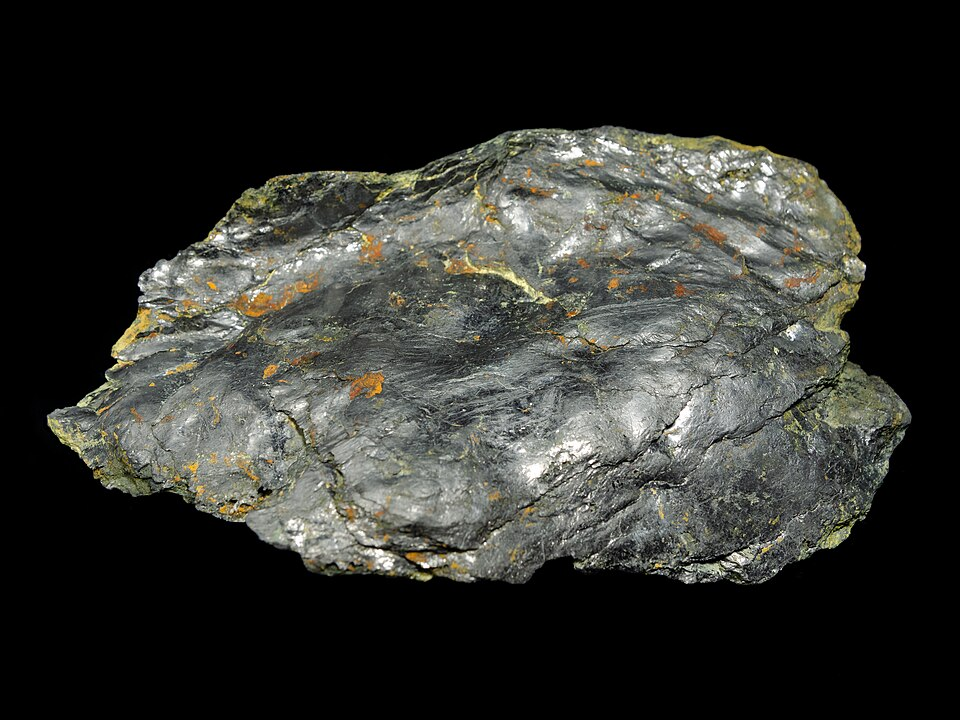
\includegraphics[width=0.36\linewidth]{images/book2/graphite.jpg}

{\small 天然石墨样品，具有金属光泽。
照片：Zbynek Burival，CC BY-SA 4.0。}
\end{omfigure}

\section{分子晶体}

\begin{definition}[分子晶体]\label{def:b1:crystals-ionic-covalent:molecular-crystal}
由分子借分子间作用力结合而成的晶体，称为
\emph{分子晶体}\index{分子晶体}，分子间作用力为范德华相互作用，
若可能还有氢键，而各分子保留自身的共价键。
例如：碘单质、干冰 \ce{CO2(s)}、冰、糖。
\end{definition}

\begin{proposition}[分子晶体的性质]\label{prop:b1:crystals-ionic-covalent:molecular}
分子晶体质地柔软，在较低温度下熔化或升华，
因为只需破坏较弱的分子间作用力；它们不导电。
\end{proposition}
\admitted

\begin{example}[冰]\label{ex:b1:crystals-ionic-covalent:ice}
在普通冰中，每个水分子与其他四个分子形成氢键，
这四个分子位于四面体顶点：其中两个借自身的氢原子，
另两个借自身的孤电子对形成氢键。这种开放的六方网络，由氢键方向所决定，
留出大量空隙：冰的密度小于液态
水，其中网络部分被破坏，分子
靠得更近。网络的六方对称性体现在
雪晶的六重形状上。
\end{example}

\begin{omfigure}
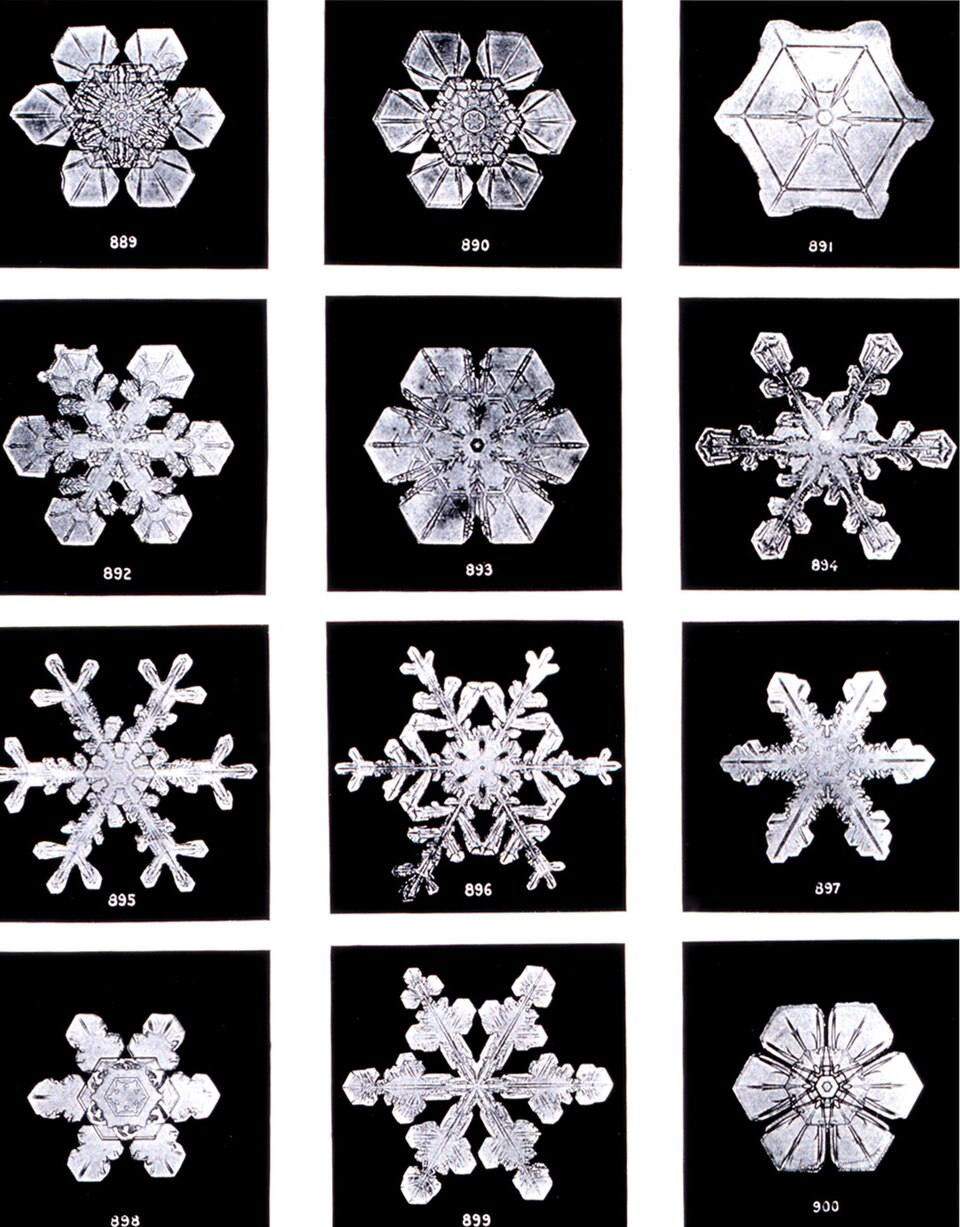
\includegraphics[width=0.38\linewidth]{images/book2/bentley-snowflakes.jpg}

{\small 威尔逊·本特利约于 1902 年拍摄的雪晶照片：每一片
都具有六重对称性，是冰中氢键六方网络
的痕迹。公有领域。}
\end{omfigure}

\section{四类固体的比较}

\begin{center}
\small
\begin{tabular}{lllll}
\hline
固体 & 粒子 & 结合力 & 性质 & 例子 \\
\hline
金属 & 阳离子、电子 & 金属键 & 导体、延展性好 & \ce{Cu}、\ce{Fe}、\ce{Na} \\
离子 & 阳离子、阴离子 & 静电作用 & 硬、脆、绝缘 & \ce{NaCl}、\ce{CaF2} \\
共价 & 原子 & 共价键 & 非常硬、熔点高 & 金刚石、\ce{SiO2} \\
分子 & 分子 & 范德瓦耳斯相互作用、氢键 & 软、熔点低 & \ce{I2}、冰 \\
\hline
\end{tabular}
\end{center}

\begin{remark}[连续过渡]\label{rem:b1:crystals-ionic-covalent:continuum}
这些分类都是理想化的。硫化锌的化学键部分为离子型，
部分为共价型，这正是其硫–锌距离短于
离子半径之和的原因；石墨层内为共价键，
层间则为分子型。电负性差
（\cref{prop:b1:periodicity:en-trend}）是判断依据：电负性差越大，
固体越偏向离子型。
\end{remark}

\section{练习}

\begin{exercise}[$\star$]\label{exo:b1:crystals-ionic-covalent:1}
在岩盐晶胞中，数出阳离子和阴离子的个数，给出
每种离子的配位数，并检验化学式 \ce{NaCl} 是否相符。
\end{exercise}

\begin{exercise}[$\star$]\label{exo:b1:crystals-ionic-covalent:2}
已知氯化铯的 $a = \qty{412.3}{pm}$，计算最短的
\ce{Cs-Cl} 距离以及每个晶胞中的化学式单元数。
\end{exercise}

\begin{exercise}[$\star$]\label{exo:b1:crystals-ionic-covalent:3}
利用半径 $r(\ce{Na+}) = \qty{102}{pm}$ 与 $r(\ce{Cl-}) =
\qty{181}{pm}$，计算 \ce{NaCl} 的半径比，并预测
阳离子的配位数。
\end{exercise}

\begin{exercise}[$\star$]\label{exo:b1:crystals-ionic-covalent:4}
判断下列物质属于金属型、离子型、共价型还是分子型：
铜、氯化钠、金刚石、碘、石英 \ce{SiO2}、冰、氟化钙。
\end{exercise}

\begin{exercise}[$\star\star$]\label{exo:b1:crystals-ionic-covalent:5}
证明岩盐结构要求 $r_+/r_- \ge \sqrt2 - 1$。
\end{exercise}

\begin{exercise}[$\star\star$]\label{exo:b1:crystals-ionic-covalent:6}
由 $a = \qty{564.1}{pm}$，计算氯化钠的密度，
（$M(\ce{NaCl}) = \qty{58.44}{g/mol}$），并与
\qty{2.17}{g/cm^3} 比较。
\end{exercise}

\begin{exercise}[$\star\star$]\label{exo:b1:crystals-ionic-covalent:7}
计算氯化铯的密度（$M = \qty{168.36}{g/mol}$，
$a = \qty{412.3}{pm}$），并与实测值 \qty{3.99}{g/cm^3} 比较。
% ledger: rho:CsCl
\end{exercise}

\begin{exercise}[$\star\star$]\label{exo:b1:crystals-ionic-covalent:8}
对于闪锌矿（$a = \qty{540.9}{pm}$，$M = \qty{97.44}{g/mol}$），计算
\ce{Zn-S} 距离和密度，并与实测值
\qty{4.04}{g/cm^3} 比较。
% ledger: rho:ZnS
\end{exercise}

\begin{exercise}[$\star\star$]\label{exo:b1:crystals-ionic-covalent:9}
石墨为六方晶胞，$a = \qty{245.6}{pm}$ 且
$c = \qty{669.6}{pm}$，含 4 个原子。计算层内
\ce{C-C} 距离（$a/\sqrt3$）、层间距离（$c/2$）以及
密度。为什么石墨的密度比金刚石小？
\end{exercise}

\begin{exercise}[$\star\star\star$]\label{exo:b1:crystals-ionic-covalent:10}
证明金刚石的堆积率为 $\pi\sqrt3/16$，并解释为什么
最硬的材料之一，其堆积率恰属最低之列。
\end{exercise}

\begin{exercise}[$\star\star\star$]\label{exo:b1:crystals-ionic-covalent:11}
硅具有金刚石结构，$a = \qty{543.1}{pm}$。计算
\ce{Si-Si} 键长、硅的共价半径以及密度
（$M = \qty{28.09}{g/mol}$），并与 \qty{2.33}{g/cm^3} 比较。
\end{exercise}

\begin{exercise}[$\star\star\star$]\label{exo:b1:crystals-ionic-covalent:12}
氯化铷中 $r(\ce{Rb+}) = \qty{152}{pm}$（六配位）与
$r(\ce{Cl-}) = \qty{181}{pm}$。半径比规则预测其为哪种结构？
常温常压下，它属于氯化钠型，其中
$a = \qty{658.1}{pm}$：检验 \ce{Rb-Cl} 距离，并说明
此处该规则为何失效。
% ledger: rion:Rb+VI, rion:Cl-VI, lat:RbCl
\end{exercise}

\section{问题：萤石、矿物与透镜}

\begin{problem}[{周末问题——萤石晶胞、其半径比、
两个相关物质（\ce{Li2O} 和金刚石），以及由其晶胞
算出的萤石密度}]
\label{pb:b1:crystals-ionic-covalent:1}
萤石 \ce{CaF2} 是一种矿物；长成的大块透明晶体可用来制作
透过紫外线的透镜。其晶胞为立方晶胞，$a =
\qty{546.3}{pm}$；\ce{Ca^{2+}} 位于面心立方晶格上，\ce{F-} 位于
四面体间隙中。半径：$r(\ce{Ca^{2+}}) = \qty{112}{pm}$（八
配位），$r(\ce{F-}) = \qty{131}{pm}$（四配位）。摩尔质量
（g/mol）：\ce{Ca} 40.08，\ce{F} 19.00，\ce{Li} 6.94，\ce{O} 16.00，\ce{C}
12.01，\ce{Si} 28.09；$N_A = \qty{6.022e23}{mol^{-1}}$。
% ledger: lat:CaF2, rion:Ca2+VIII, rion:F-IV, aw:Ca, aw:F, aw:Li, aw:O,
% aw:C, aw:Si, const:NA

\medskip
\noindent\textbf{第一部分——晶胞。}
\begin{enumerate}
  \item 给出晶胞中 \ce{Ca^{2+}} 离子的位置，并
        统计它们的个数。
  \item 晶胞中含有多少个四面体间隙？推出
        \ce{F-} 离子的个数，并检验化学式。
  \item \ce{F-} 的配位数是多少？\ce{Ca^{2+}} 的配位数是多少？
  \item 计算最短的 \ce{Ca-F} 距离。
  \item 将其与离子半径之和比较。
  \item 计算最短的 \ce{F-F} 距离，并
        判断阴离子是否相接触。
\end{enumerate}

\medskip
\noindent\textbf{第二部分——半径比。}
\begin{enumerate}[resume]
  \item 计算 $x = r_+/r_-$。
  \item 半径比规则允许阳离子取何种配位数？
  \item 为什么 \ce{CaF2} 不能取氯化铯结构，
        尽管其阳离子为 8 配位？
  \item 将萤石描述为 \ce{F-} 构成的简单立方排列，其中
        \ce{Ca^{2+}} 位于一半小立方体的中心。
  \item 计算萤石的堆积率。
\end{enumerate}

\medskip
\noindent\textbf{第三部分——两个近亲。}
氧化锂 \ce{Li2O} 为反萤石结构，$a = \qty{461.9}{pm}$；
$r(\ce{Li+}) = \qty{59}{pm}$（四个近邻），$r(\ce{O^{2-}}) =
\qty{142}{pm}$（八个近邻）。金刚石：$a = \qty{356.7}{pm}$。
% ledger: lat:Li2O, rion:Li+IV, rion:O2-VIII, rho:Li2O, lat:C-diamond
\begin{enumerate}[resume]
  \item \ce{O^{2-}} 和 \ce{Li+} 离子在反萤石
        晶胞中分别位于何处？
  \item 计算 \ce{Li-O} 距离，并与
        半径之和比较。
  \item 计算 \ce{Li2O} 的密度，并与实测值
        \qty{2.01}{g/cm^3} 比较。
  \item 哪一种离子型结构的离子位置排布与
        金刚石相同？
  \item 计算 \ce{C-C} 键长及金刚石的密度。
  \item 为什么金刚石的堆积程度远低于萤石，
        尽管其原子占据的是同一类位置？
\end{enumerate}

\medskip
\noindent\textbf{第四部分——萤石的密度。}
\begin{enumerate}[resume]
  \item 计算 \ce{CaF2} 的摩尔质量。
  \item 计算一个晶胞的质量。
  \item 计算一个晶胞的体积，单位为 \unit{cm^3}。
  \item 若每一百个晶胞中有一个 \ce{F-} 位点为空位，
        密度会受到什么影响？
  \item 由晶胞计算萤石的密度，并与
        实测值 \qty{3.18}{g/cm^3} 比较。
\end{enumerate}
% ledger: rho:CaF2
\end{problem}
